\chapter{服务治理与监控}
\section{服务网络架构与传统网络架构对比与分析}
在现代微服务架构中,服务网络架构起着至关重要的作用。与传统的网络架构相比,服务网络架构引入了许多新的概念和技术,以更好地满足微服务应用的需求。本节将对服务网络架构与传统网络架构进行对比与分析,并探讨它们的优势和劣势。

\subsection{传统网络架构}

传统的网络架构通常基于三层模型,即应用层、传输层和网络层。在这种架构中,应用程序通过传输层协议(如 TCP 或 UDP)进行通信,并依赖于网络层协议(如 IP)进行数据传输。这种架构主要面向主机和网络之间的通信,而不太适用于微服务架构中的服务间通信。

在传统网络架构中,通信通常是基于主机和端口的,服务的位置和可用性对应用程序来说是透明的。这导致了以下一些问题:

\begin{itemize}
	\item \textbf{单点故障(SPOF):} 传统架构中的应用程序通常会直接连接到特定主机和端口。如果该主机或端口不可用,应用程序将无法正常工作,导致单点故障。
	\item \textbf{服务发现困难: }应用程序需要手动配置目标服务的主机和端口信息,这在大规模微服务系统中变得非常繁琐和复杂。随着服务数量的增加和动态变化,手动管理服务发现变得几乎不可行。
	\item \textbf{无法适应动态环境:} 传统架构很难适应动态环境中服务的频繁启动、停止和迁移。应用程序需要实时感知服务的变化,并相应地更新配置信息,这对于开发人员来说是一项巨大的挑战。
\end{itemize}

\subsection{服务网络架构}

服务网络架构通过引入服务代理和服务注册等概念,提供了一种更灵活、可扩展和可靠的服务间通信方式。在服务网络架构中,服务通过代理进行通信,代理负责处理服务发现、负载均衡、故障处理等任务。

以下是服务网络架构的一些关键概念和技术:

\begin{itemize}
	\item \textbf{服务代理: }服务代理是位于服务之间的中间层,它处理服务发现、负载均衡、熔断等功能。代理与每个服务建立连接,并代表应用程序进行通信,从而解耦了应用程序与具体服务之间的直接依赖关系。
	\item \textbf{服务注册: }服务注册是将服务实例的元数据(如主机和端口信息)注册到中心注册表中的过程。注册表充当服务发现的中心,应用程序可以查询注册表来获取目标服务的位置和可用性信息。
	\item \textbf{负载均衡: }服务代理可以根据负载均衡算法将请求分发到多个服务实例中,以实现负载均衡和高可用性。常见的负载均衡算法包括轮询、随机和加权轮询等。
	\item \textbf{熔断:} 熔断是一种故障处理机制,当目标服务发生故障或超过一定阈值时,服务代理会中断对该服务的请求,以避免故障的扩散和影响到其他服务。
\end{itemize}

服务网络架构相对于传统网络架构具有许多优势:

\begin{itemize}
	\item \textbf{高可用性和弹性:} 通过负载均衡和熔断等机制,服务网络架构能够提供高可用性和弹性,即使在某些服务实例故障的情况下,应用程序仍然可以正常工作。
	\item \textbf{动态服务发现:} 服务注册和服务发现机制使得应用程序能够动态地发现和连接到目标服务,无需手动配置主机和端口信息。这对于大规模微服务系统的管理和扩展非常重要。
	\item \textbf{灵活的部署和扩展: }服务网络架构使得服务的部署和扩展变得更加灵活和简化。服务可以独立部署和扩展,而无需修改应用程序的配置。
\end{itemize}

综上所述,服务网络架构相对于传统网络架构在微服务架构中具有许多优势,并且能够更好地满足微服务应用的需求。通过引入服务代理、服务注册和负载均衡等概念,服务网络架构实现了服务之间的解耦和动态发现,从而提高了系统的可靠性、可扩展性和可维护性。

本节主要实现一些监控(Prometheus)、追踪(Zipkin)、数据可视化工具(Grafana)和服务拓扑结构(Kiali)。
\section{熔断、限流、认证、授权的问题分析}
\subsection{熔断}
熔断是一种故障处理机制,用于保护系统免受服务故障的影响。当服务的错误率超过预定阈值时,熔断机制将临时中断对该服务的请求,以避免故障的扩散和对系统性能的负面影响。

监控熔断的关键是收集并分析与服务调用相关的指标。这些指标可以包括请求错误率、响应时间、失败率等。通过监控这些指标,可以及时检测到服务的故障情况,并触发熔断机制。

在解决熔断问题时,可以采取以下几个可行的解决思路:
\begin{itemize}
	\item \textbf{设置故障阈值}: 根据服务的性能和可靠性需求,设置适当的故障阈值。当服务的错误率超过该阈值时,触发熔断机制。
	\item \textbf{实施回退策略:} 当服务被熔断时,可以采取回退策略,例如返回默认值或从缓存中获取数据。这样可以确保在服务不可用时,仍能提供一定程度的功能。
	\item \textbf{自动恢复机制:} 一旦服务的错误率降低到可接受的水平,熔断机制应自动恢复服务,并逐渐增加请求量,以确保服务的可用性。
	\item \textbf{监控和报警系统}: 配置监控和报警系统来实时监测服务的错误率和熔断状态。当触发熔断时,及时通知开发团队并采取相应的措施。
\end{itemize}
\subsection{限流}
限流是一种保护系统免受过载的机制,用于限制对服务的并发请求量或吞吐量。通过限制请求的数量,可以防止服务过载和资源耗尽。

监控限流的关键是收集和分析与请求量和资源利用率相关的指标。这些指标可以包括并发请求数、吞吐量、平均响应时间等。通过监控这些指标,可以及时发现并处理潜在的请求过载问题。

在解决限流问题时,可以考虑以下几个解决思路:
\begin{itemize}
	\item \textbf{设置请求配额: }根据系统的容量和资源限制,设置每个服务的最大并发请求数或吞吐量。超过限制的请求将被拒绝或延迟处理。
	\item \textbf{实施排队机制: }当请求量超过系统处理能力时,可以将请求放入队列中,并按照一定的策略进行处理。这样可以有效控制请求的处理速率,避免资源耗尽。
	\item \textbf{动态调整限流策略: }根据系统负载和性能指标,动态调整限流策略。例如,在高负载时降低限流阈值,以避免系统过载;在低负载时适当提高限流阈值,以提高系统的利用率。
	\item \textbf{监控和报警系统: }配置监控和报警系统来实时监测请求量和限流状态。当触发限流时,及时通知开发团队并采取相应的措施。
\end{itemize}

\subsection{认证与授权}
认证与授权是保护系统安全和数据机密性的关键机制。认证用于验证用户身份,而授权用于确定用户对系统资源的访问权限。

监控认证与授权的关键是收集和分析与用户身份验证和资源访问相关的指标。这些指标可以包括登录失败次数、授权错误次数、授权访问成功率等。通过监控这些指标,可以及时发现安全漏洞和异常访问行为。

在解决认证与授权问题时,可以采取以下几个解决思路:
\begin{itemize}
	\item \textbf{多因素认证: }引入多因素认证机制,例如使用密码和验证码的组合,以提高身份验证的安全性。
	
	\item \textbf{使用安全令牌: }使用安全令牌(如 JWT)进行认证和授权,以避免在每次请求时都进行身份验证和授权。
	
	\item \textbf{实施权限管理: }管理用户的访问权限,并确保只有授权用户能够访问系统的特定资源。
	
	\item \textbf{监控和审计系统: }配置监控和审计系统来记录认证和授权的操作日志,并定期进行审查和分析,以发现异常访问行为。
\end{itemize}
\subsection{链路追踪}
链路追踪是一种分布式系统的监控技术,用于跟踪和分析请求在不同服务之间的流动和处理情况,以便识别和解决潜在的性能瓶颈和故障。

监控链路追踪的关键是收集和分析与请求流程、服务调用和响应时间相关的指标。这些指标可以包括请求的唯一标识符、请求的起始时间和结束时间、每个服务的处理时间等。通过监控这些指标,可以可视化请求的流程并分析服务间的调用关系。

在解决链路追踪问题时,可以考虑以下几个解决思路:
\begin{itemize}
	\item \textbf{使用分布式追踪系统: }集成分布式追踪系统(如 Jaeger、Zipkin)来收集和分析请求的链路信息。这些系统可以自动记录和跟踪请求在不同服务之间的流动情况。
	
	\item \textbf{添加唯一标识符:} 在每个请求中添加唯一标识符,并将其传递给后续的服务。这样可以跟踪请求在不同服务间的流动,并分析每个服务的处理时间。
	
	\item \textbf{可视化链路图: }根据收集的链路数据,生成可视化的链路图,显示请求在不同服务间的流动和处理情况。这样可以帮助开发团队快速定位性能瓶颈和故障点。
	
	\item \textbf{分析和优化: }基于链路追踪数据进行分析,找出潜在的性能瓶颈和故障点,并采取相应的优化措施,以提高系统的性能和可靠性。
\end{itemize}
\subsection{可观察性与指标}
由于采用了 sidecar 部署模式,即 Envoy 代理运行在应用实例旁边并拦截流量,这些代理也收集指标。

Envoy 代理收集的指标可以帮助我们获得系统状态的可见性。获得系统的这种可见性是至关重要的,因为我们需要了解正在发生的事情,并授权运维人员对应用程序进行故障排除、维护和优化。

Istio 生成三种类型的遥测数据,为网格中的服务提供可观察性\cite{istio-data}:
\begin{itemize}
	\item 指标度量(Metric)
	\item 分布式追踪
	\item 访问日志
\end{itemize}
Istio 基于四个黄金信号生成指标:延迟、流量、错误和饱和度。
\begin{itemize}
	\item 延迟表示服务一个请求所需的时间。这个指标应该分成成功请求(如 HTTP 200)和失败请求(如 HTTP 500)的延迟。
	\item 流量是衡量对系统的需求有多大,它是以系统的具体指标来衡量的。例如,每秒的 HTTP 请求,或并发会话,每秒的检索量,等等。
	\item 错误用来衡量请求失败的比率(例如 HTTP 500)。
	\item 饱和度衡量一个服务中最紧张的资源有多满。例如,线程池的利用率。
\end{itemize}
这些指标是在不同的层面上收集的,首先是最细的,即 Envoy 代理层面,然后是服务层面和控制平面的指标。本节接下来的部分针对服务拓扑发现与链路追踪、性能监控与可观测性两个层面配置和使用各种可观察性、分布式追踪、数据可视化工具。
\section{性能监控与可观测性}
在性能监控和可观测性分析中,Grafana和Prometheus是两个重要的工具,它们通常被一起使用来构建全面的监控和分析系统。

Prometheus是一个开源的监控系统和时间序列数据库,专门用于收集、存储和查询系统的指标数据。它支持灵活的数据模型和查询语言,能够高效地处理大量的时间序列数据。Prometheus采用了基于拉取的方式,周期性地从各个目标(如应用程序、服务、主机等)收集指标数据,并将其存储在本地的时间序列数据库中。它还提供了丰富的查询语言和表达式,用于实时监控和分析指标数据,例如计算平均值、聚合数据、设置报警规则等。

Grafana则是一个强大的数据可视化平台,用于展示和分析来自不同数据源的监控指标数据。Grafana支持多种数据源,其中包括Prometheus。它提供了直观的用户界面,用户可以根据需要创建自定义的仪表盘和面板,将不同数据源的指标数据可视化呈现出来。通过Grafana,用户可以轻松地创建图表、图形、表格等各种可视化元素,以实时、直观的方式展示系统的性能指标和趋势。此外,Grafana还支持设置报警规则和通知机制,以便在系统达到预设的阈值时发送警报通知。

综合使用Prometheus和Grafana,可以建立一个完整的性能监控和可观测性分析系统。Prometheus负责数据的收集、存储和查询,而Grafana则负责将这些数据进行可视化展示和分析。用户可以通过Grafana创建个性化的仪表盘,实时监控系统的各项指标,并根据需要进行深入的数据分析和性能优化。这样的组合能够帮助用户更好地了解系统的运行状态、发现潜在的问题,并及时采取相应的措施来提高系统的性能和稳定性。
\subsection{Prometheus 的配置与使用}
Prometheus 是一个开源的监控系统和时间序列数据库,最初由 SoundCloud 开发并于2012年发布。它专为高度动态的分布式环境而设计,可以帮助用户监控系统和服务的性能指标、告警状态以及记录事件数据。

Prometheus 通过收集和存储时间序列数据来实现监控功能。它支持多种数据模型和查询语言,可以有效地存储大规模的时间序列数据,并提供强大的查询和聚合功能。Prometheus 使用拉取模型,周期性地从目标系统中获取指标数据,同时也支持推送模型,允许目标系统将数据主动推送给 Prometheus。

Prometheus 提供了灵活的告警规则配置,可以基于采集的指标数据定义自定义的告警条件,并在触发告警时发送通知。它还具有强大的可视化能力,通过内置的图形界面和集成的 Grafana 工具,用户可以实时监控和分析指标数据,创建仪表板和报表来展示系统的状态和趋势。

在 Istio 中,Prometheus 被用于记录指标,跟踪 Istio 和服务网格中应用程序的健康状况。它可以与 Istio 的各个组件集成,帮助用户实现对服务的监控、度量和告警。

要安装 Prometheus,我们可以使用 Istio 安装包中 /samples/addons 文件夹中的示例安装。
\begin{lstlisting}[language=bash][language=bash, caption={安装 Prometheus}]
[root@k8scloude1 ~]# cd istio-1.14.3/
[root@k8scloude1 istio-1.14.3]# cd samples/addons/
[root@k8scloude1 addons]# vim prometheus.yaml
\end{lstlisting}
可以看到安装 Prometheus 需要用到两个镜像:jimmidyson/configmap-reload:v0.5.0 和 prom/prometheus:v2.31.1
\begin{lstlisting}[language=bash][language=bash]
# 提前在 Kubernetes 的 worker 节点拉取所需镜像,以 k8scloude2 节点为例
[root@k8scloude2 ~]# docker pull jimmidyson/configmap-reload:v0.5.0
[root@k8scloude2 ~]# docker pull prom/prometheus:v2.31.1
\end{lstlisting}
安装 Prometheus:
\begin{lstlisting}[language=bash][language=bash]
[root@k8scloude1 addons]# kubectl apply -f prometheus.yaml
serviceaccount/prometheus created
configmap/prometheus created
clusterrole.rbac.authorization.k8s.io/prometheus created
clusterrolebinding.rbac.authorization.k8s.io/prometheus created
service/prometheus created
deployment.apps/prometheus created
\end{lstlisting}
检查 Prometheus 是否成功部署
\begin{lstlisting}[language=bash][language=bash]	
[root@k8scloude1 addons]# kubectl get deploy -n istio-system
NAME                   READY   UP-TO-DATE   AVAILABLE   AGE
istio-egressgateway    1/1     1            1           62m
istio-ingressgateway   1/1     1            1           62m
istiod                 1/1     1            1           62m
prometheus             1/1     1            1           12s
\end{lstlisting}
检查 Prometheus 运行状态
\begin{lstlisting}[language=bash][language=bash]	
[root@k8scloude1 ~]# kubectl get pod -n istio-system -o wide
NAME                                    READY   STATUS    RESTARTS   AGE   IP            NODE    NOMINATED NODE   READINESS GATES
istio-egressgateway-5f864bf78f-n4bs4    1/1     Running   0          62m   10.244.2.14   node2   <none>           <none>
istio-ingressgateway-78c7bbfc7c-wbtdd   1/1     Running   0          62m   10.244.2.15   node2   <none>           <none>
istiod-fcb96b864-87gcx                  1/1     Running   0          62m   10.244.1.11   node1   <none>           <none>
prometheus-6956c8c6c5-6zc94             2/2     Running   0          48s   10.244.1.12   node1   <none>           <none>
b-kz5sd                 1/1     Running   10         8d    10.244.112.137   k8scloude2
\end{lstlisting}
查看 Istio 系统中的 Prometheus 服务类型为 ClusterIP,无法从外部环境访问,修改 Prometheus 这个 service 的类型为 NodePort,这样外部环境就可以访问 Prometheus 。将 "type: ClusterIP" 修改为 "type: NodePort"
\begin{lstlisting}[language=bash][language=bash]
	kubectl edit service prometheus -n istio-system
\end{lstlisting}
\begin{lstlisting}[language=bash]
spec:
clusterIP: 10.102.117.137
clusterIPs:
- 10.102.117.137
internalTrafficPolicy: Cluster
ipFamilies:
- IPv4
ipFamilyPolicy: SingleStack
ports:
- name: http
port: 9090
protocol: TCP
targetPort: 9090
selector:
app: prometheus
component: server
release: prometheus
sessionAffinity: None
type: NodePort
status:
loadBalancer: {}
\end{lstlisting}
现在 Prometheus 这个 service 的类型为 NodePort,浏览器输入物理机 IP:pod端口号 即可访问 Prometheus 网页了
因为k8scloude1地址为192.168.210.168,所以我们可以在浏览器中打开 http://192.168.210.168:30225/,进入 Prometheus 仪表盘,输入istio\_requests\_total之后,点击Execute执行,就可以看到收集到的数据,如下图所示:

\begin{figure}[htb]
	\centering
	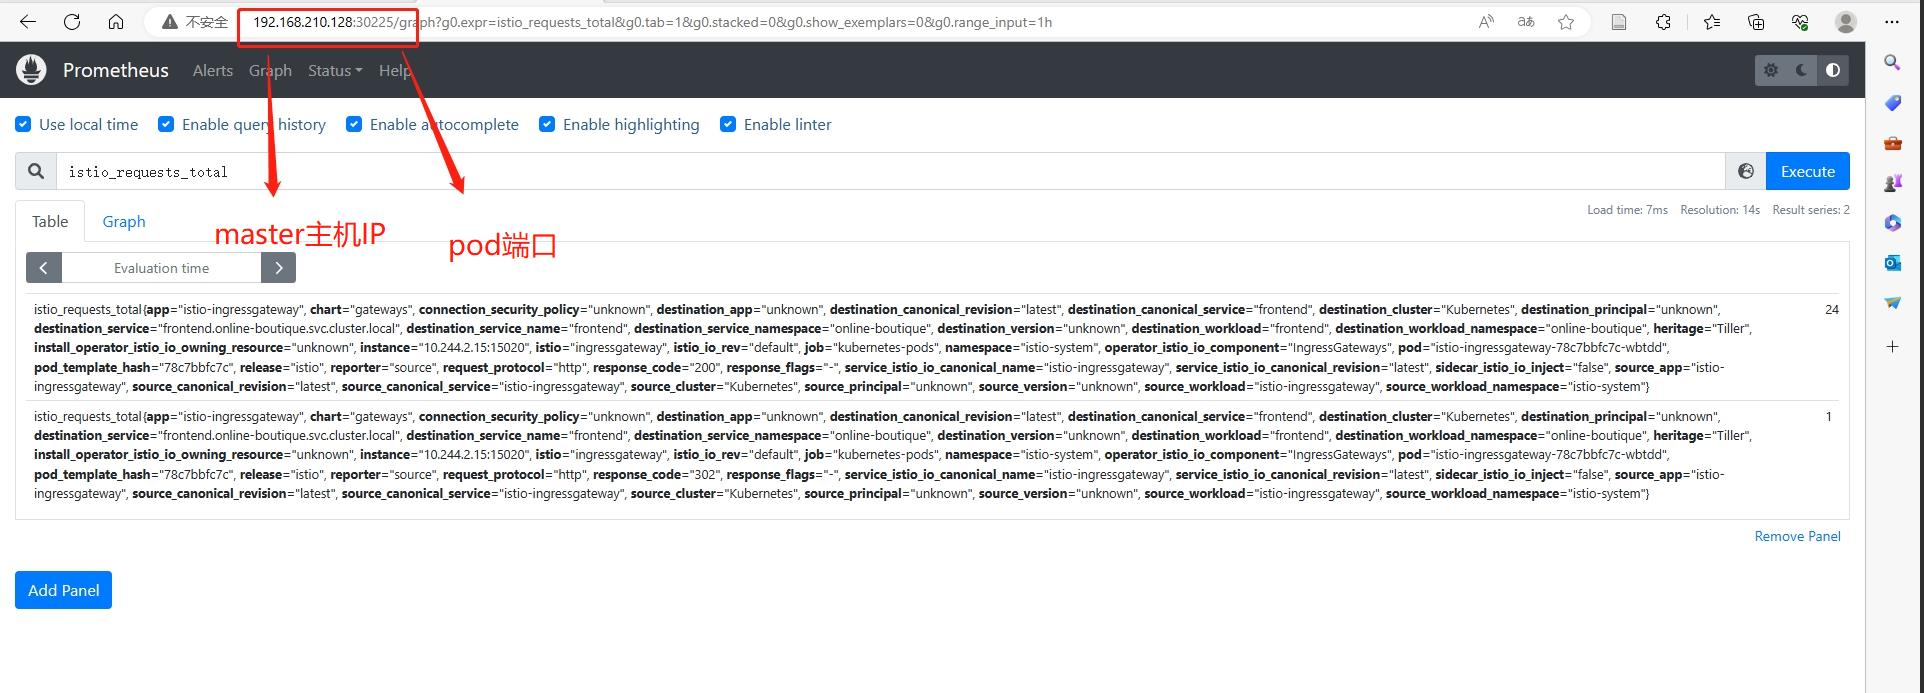
\includegraphics[width=1.0\textwidth]{figures/chapter2/prometheus.png}
	\caption{Prometheus监控仪表盘与使用}
	\label{fig:3-Prometheus监控仪表盘与使用}
\end{figure}
下面是一个来自 Prometheus 用户界面的示例元素:
\begin{lstlisting}[language=bash]
istio_requests_total{app="istio-ingressgateway", chart="gateways", connection_security_policy="unknown", destination_app="unknown", destination_canonical_revision="latest", destination_canonical_service="frontend", destination_cluster="Kubernetes", destination_principal="unknown", destination_service="frontend.online-boutique.svc.cluster.local", destination_service_name="frontend", destination_service_namespace="online-boutique", destination_version="unknown", destination_workload="frontend", destination_workload_namespace="online-boutique", heritage="Tiller", install_operator_istio_io_owning_resource="unknown", instance="10.244.2.15:15020", istio="ingressgateway", istio_io_rev="default", job="kubernetes-pods", namespace="istio-system", operator_istio_io_component="IngressGateways", pod="istio-ingressgateway-78c7bbfc7c-wbtdd", pod_template_hash="78c7bbfc7c", release="istio", reporter="source", request_protocol="http", response_code="200", response_flags="-", service_istio_io_canonical_name="istio-ingressgateway", service_istio_io_canonical_revision="latest", sidecar_istio_io_inject="false", source_app="istio-ingressgateway", source_canonical_revision="latest", source_canonical_service="istio-ingressgateway", source_cluster="Kubernetes", source_principal="unknown", source_version="unknown", source_workload="istio-ingressgateway", source_workload_namespace="istio-system"}
\end{lstlisting}
\subsection{Grafana 的配置与使用}
Grafana是一个开源的数据可视化和监控平台。它提供了丰富的数据查询、可视化和报警功能,可用于实时监控和分析各种数据源,包括时间序列数据、日志数据和数据库数据等。Grafana支持多种数据源,如Prometheus、InfluxDB、Elasticsearch等,可以根据需求创建自定义的仪表盘和面板,以便直观地展示数据指标和趋势。Grafana广泛应用于DevOps、系统监控、应用性能分析和可视化等领域,帮助用户实时监控系统状态、分析性能问题,并支持决策和故障排除。

运行以下命令来部署 Grafana 和预配置的仪表盘:
\begin{lstlisting}[language=bash][language=bash]
kubectl apply -f grafana.yaml
% 查看 Istio 系统中的 Pod
kubectl get pod -n istio-system
% 查看 Grafana 这个 service 的类型为 ClusterIP,无法从外部环境访问
kubectl get service -n istio-system
% 修改 Grafana 这个 service 的类型为 NodePort,这样外部环境就可以访问 Grafana
% 将 "type: ClusterIP" 修改为 "type: NodePort"
kubectl edit service grafana -n istio-system
% 现在 Grafana 这个 service 的类型为 NodePort,浏览器输入物理机 IP:31092 即可访问 Grafana 网页
kubectl get service -n istio-system
\end{lstlisting}

k8scloude1 机器的地址为 192.168.210.128,我们可以在浏览器中打开 \url{http://192.168.210.128:30729},进入 Grafana,点击搜索框和 istio 文件夹,查看已安装的仪表盘,如下图所示:
\begin{figure}[H]
	\centering
	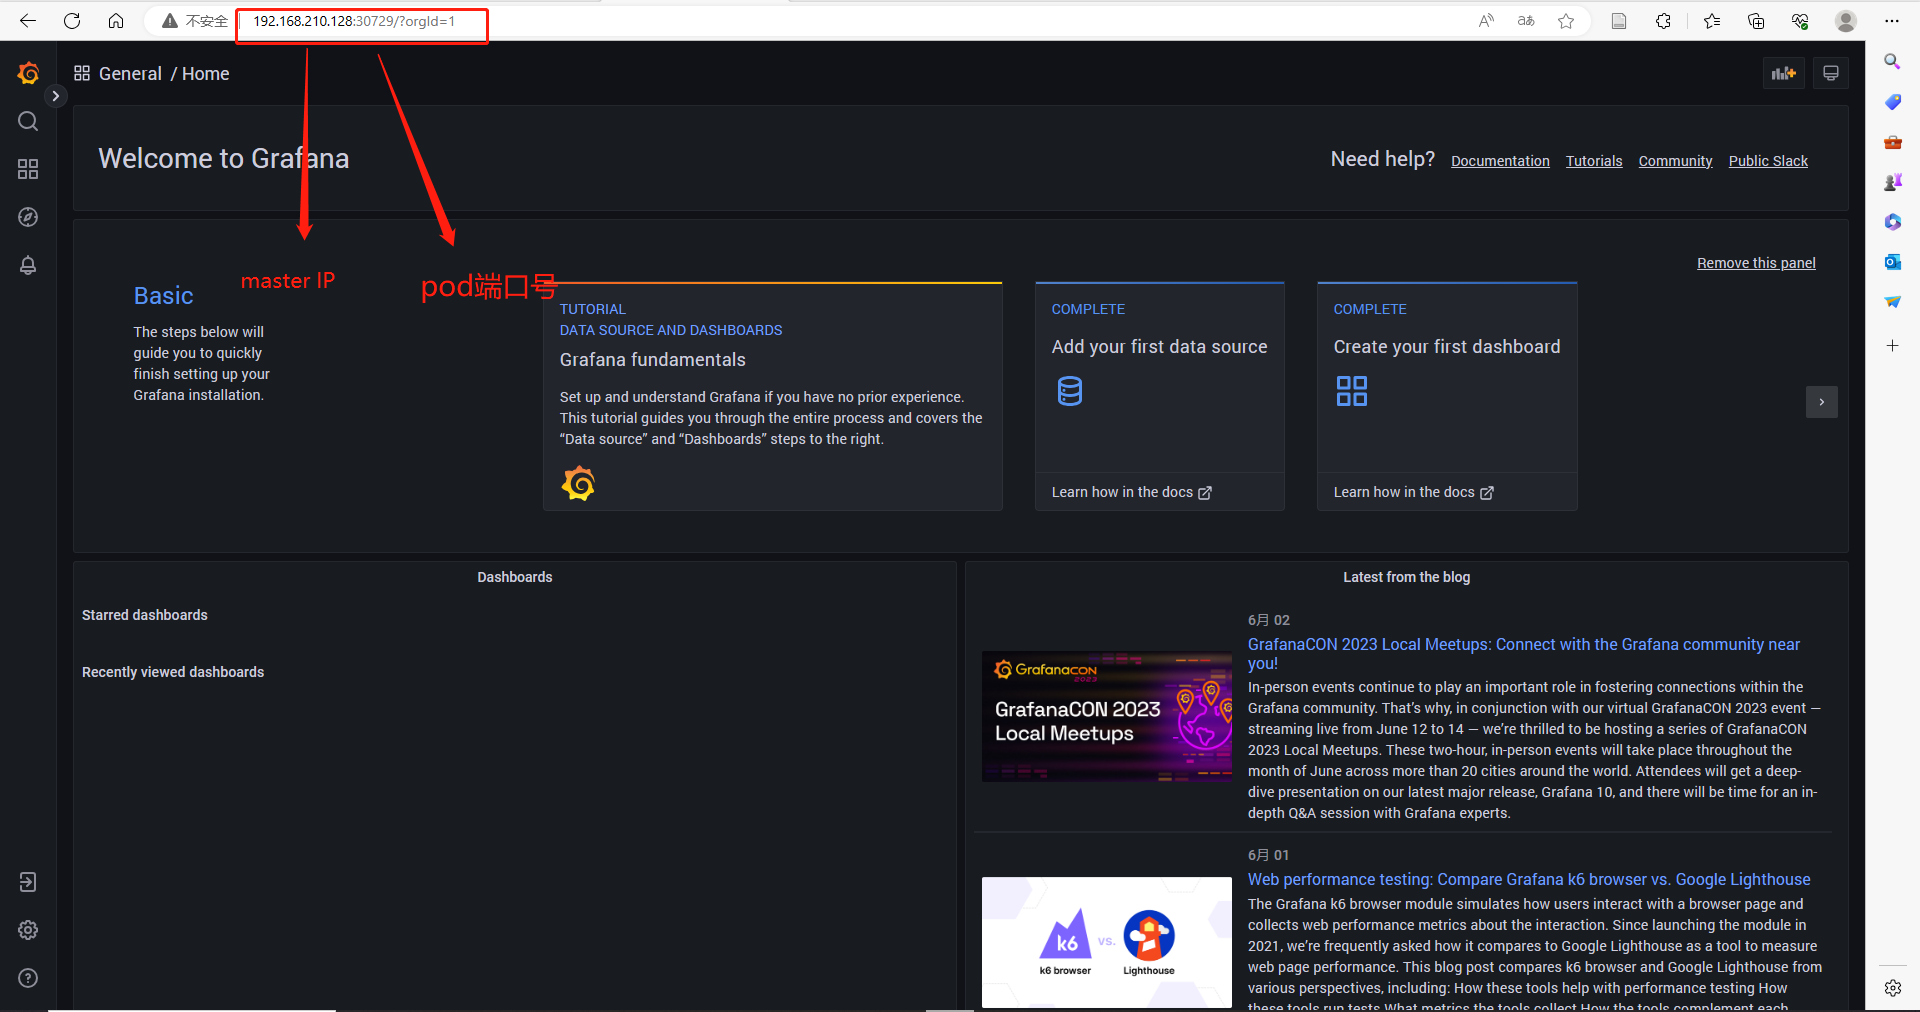
\includegraphics[width=1.0\textwidth]{figures/chapter2/grafana.png}
	\caption{Grafana监控仪表盘与使用}
	\label{fig:3-Grafana监控仪表盘与使用}
\end{figure}
Istio Grafana 安装时预配置了以下仪表盘:

Istio 控制平面仪表盘(Istio Control Plane Dashboard)可以监控 Istio 控制平面的健康和性能,展示控制平面的资源使用情况(内存、CPU、磁盘、Go routines),以及关于 Pilot、Envoy 和 Webhook 的信息。
\begin{figure}[H]
	\centering
	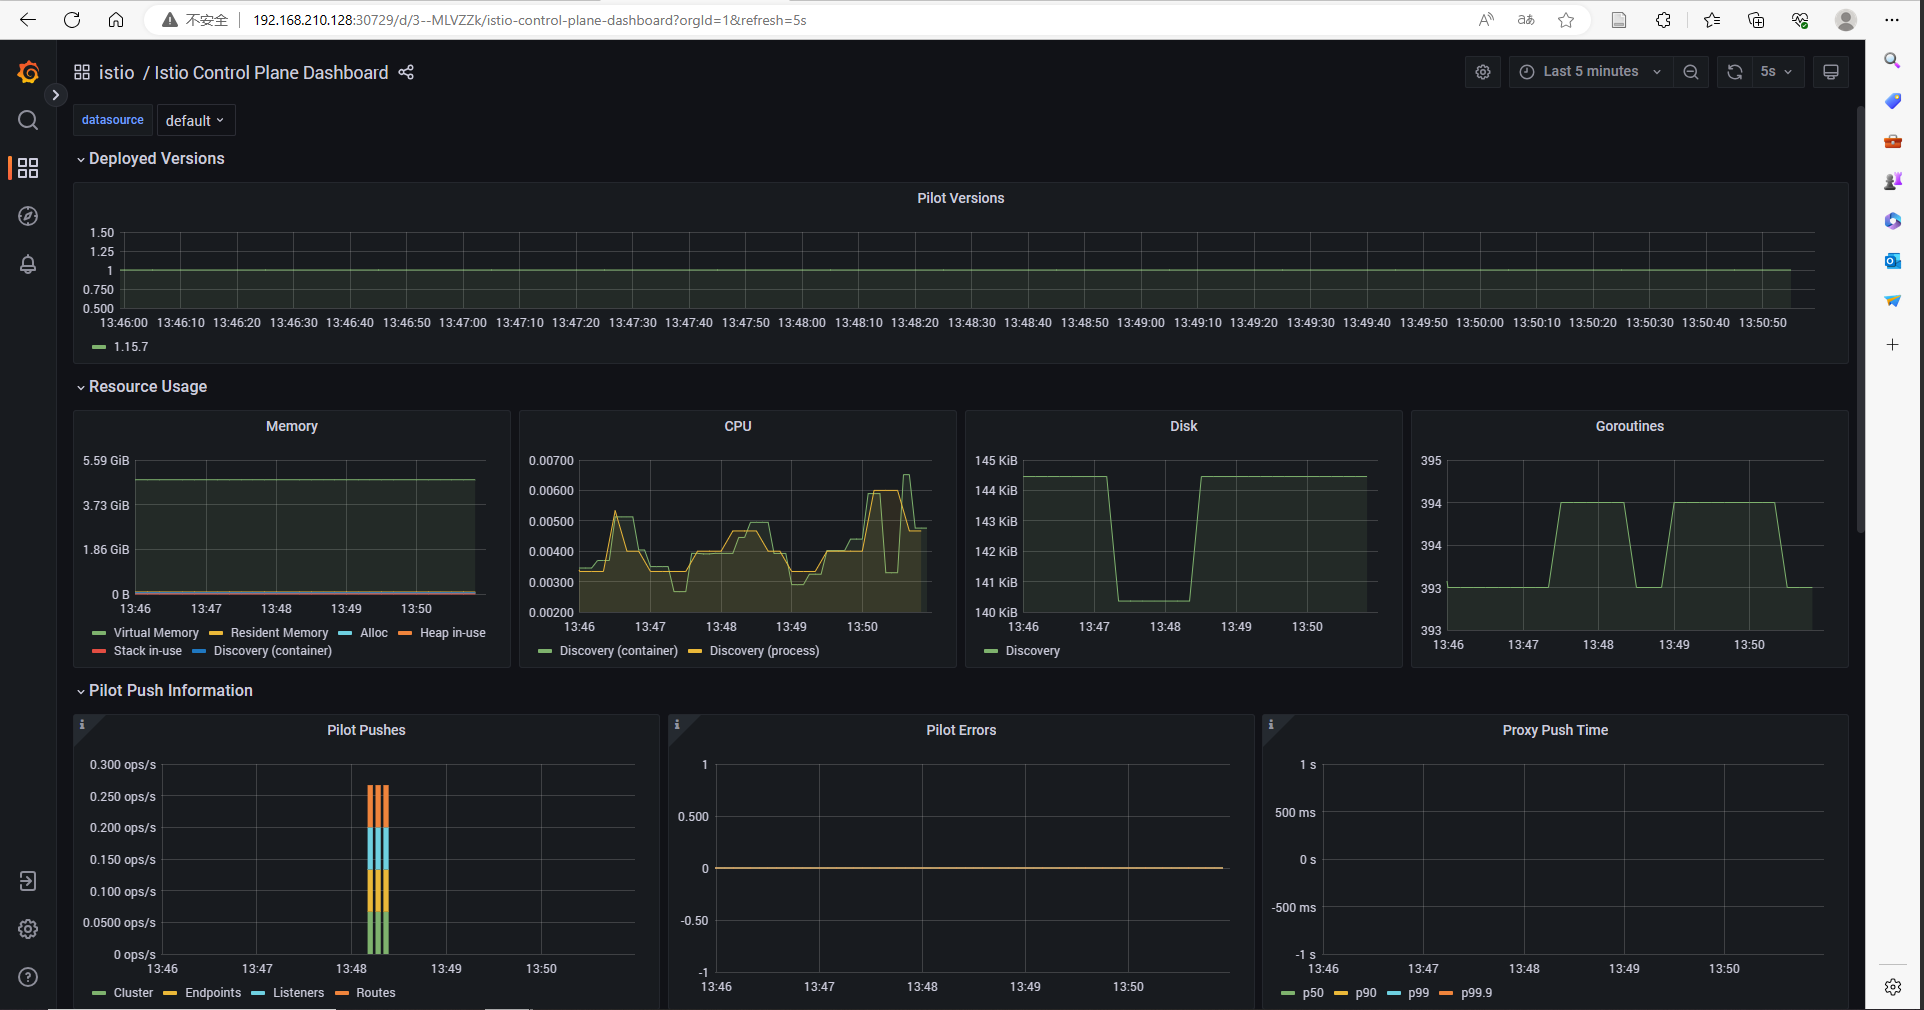
\includegraphics[width=1.0\textwidth]{figures/chapter2/CPA.png}
	\caption{Istio 控制平面仪表盘(Istio Control Plane Dashboard)}
	\label{fig:3-Istio 控制平面仪表盘(Istio Control Plane Dashboard)}
\end{figure}
Istio 网格仪表盘(Istio Mesh Dashboard)提供了在网格中运行的所有服务的概览。仪表盘包括全局请求量、成功率以及 4xx 和 5xx 响应的数量。
\begin{figure}[H]
	\centering
	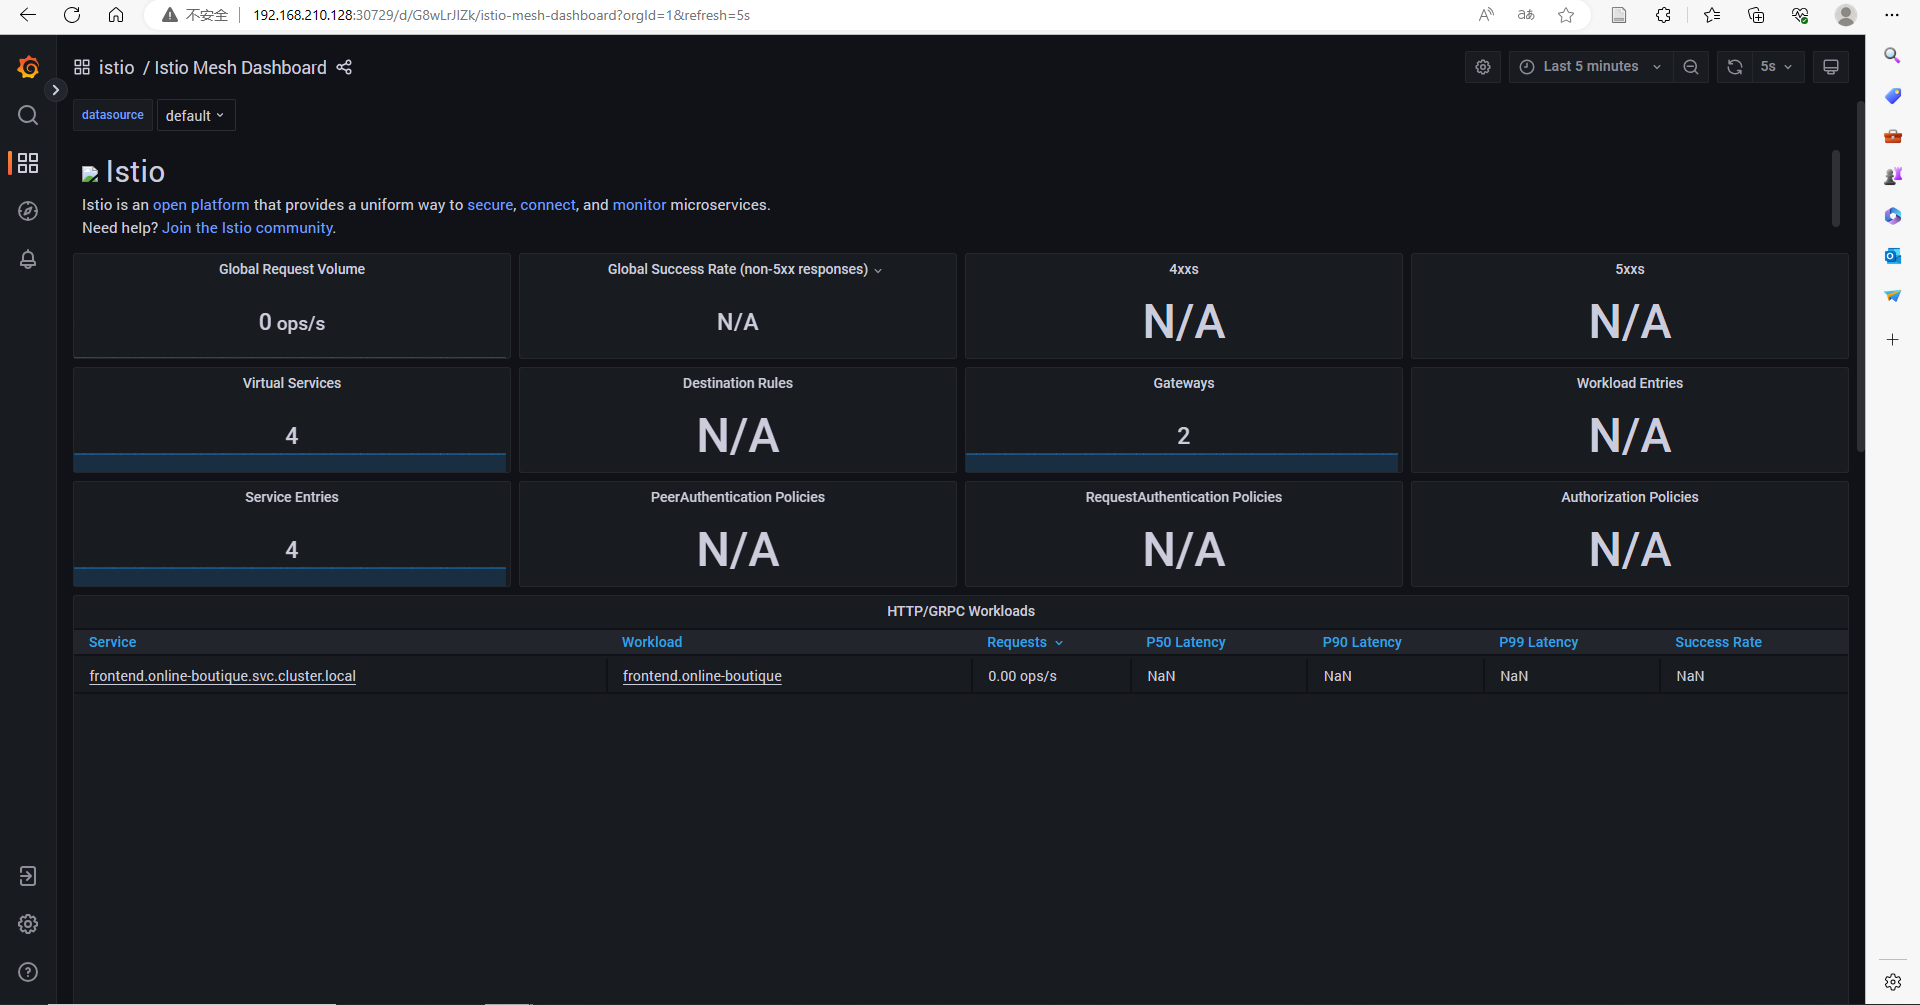
\includegraphics[width=1.0\textwidth]{figures/chapter2/MD.png}
	\caption{Istio 网格仪表盘(Istio Mesh Dashboard)}
	\label{fig:3-Istio 网格仪表盘(Istio Mesh Dashboard)}
\end{figure}
Istio 性能仪表盘(Istio Performance Dashboard)展示了 Istio 主要组件在稳定负载下的资源利用率。
\begin{figure}[H]
	\centering
	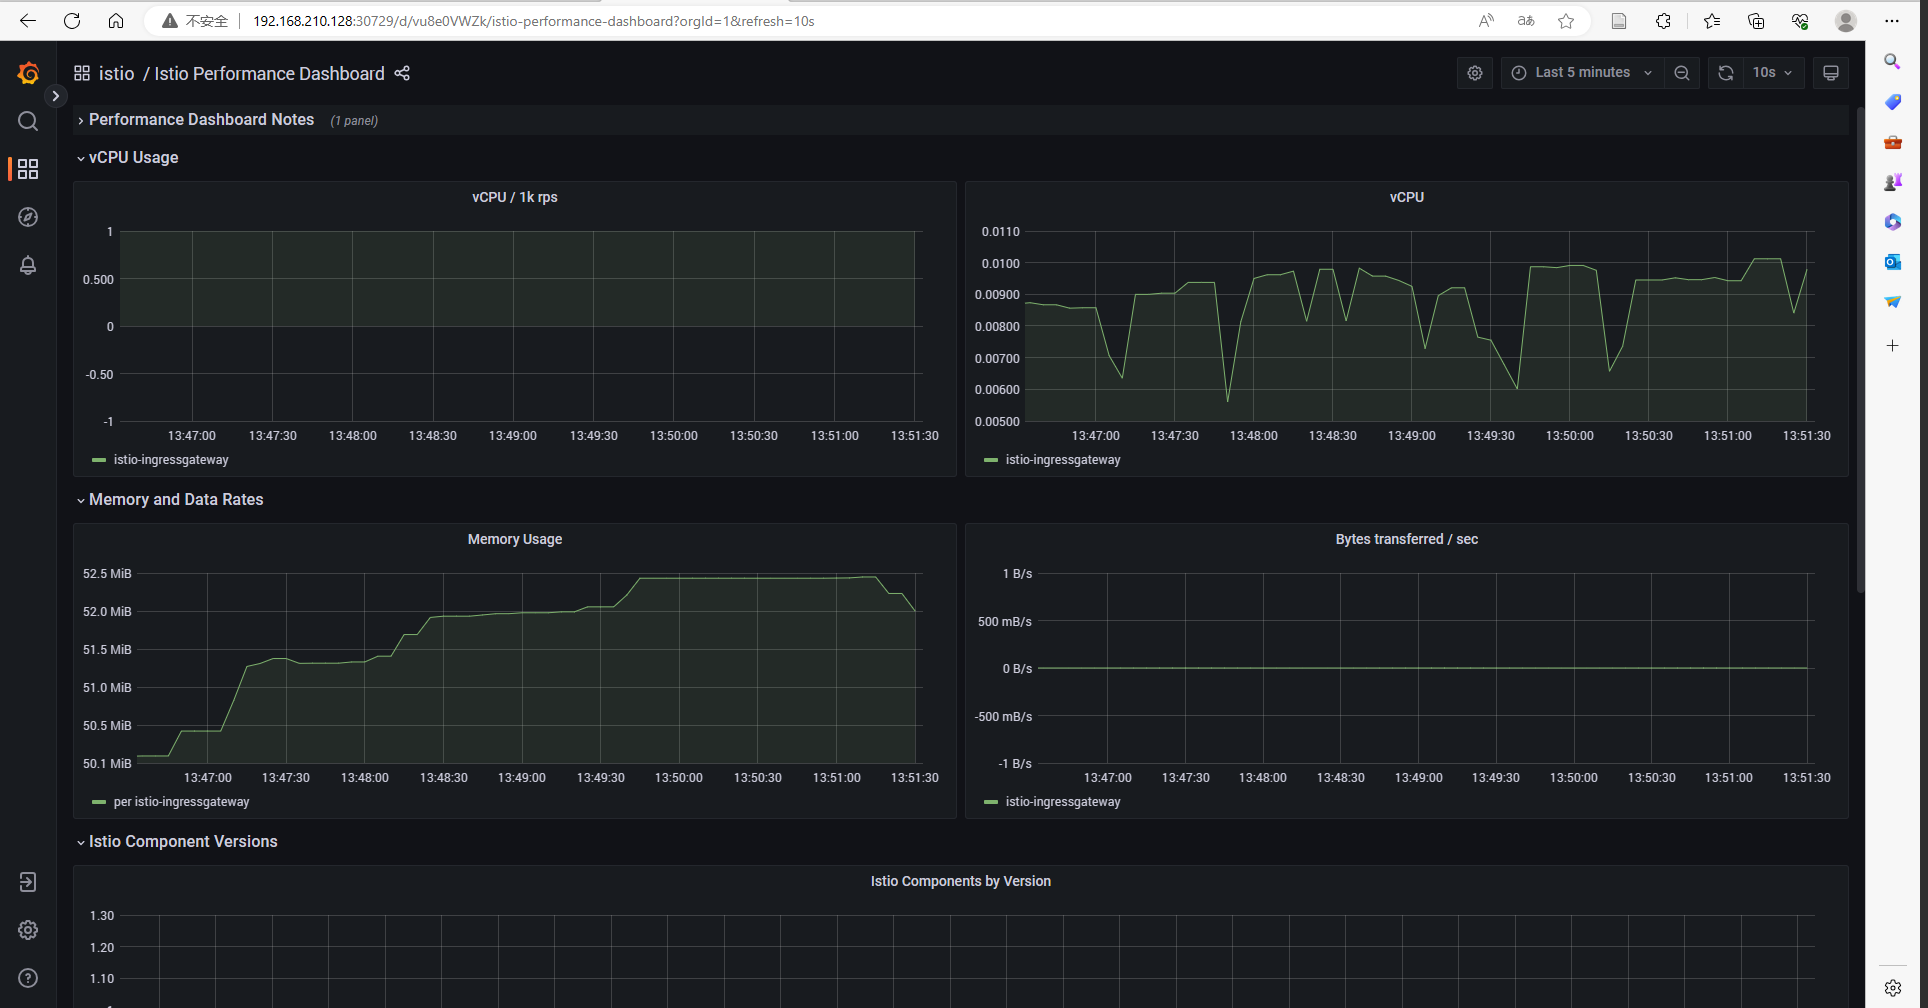
\includegraphics[width=1.0\textwidth]{figures/chapter2/PD.png}
	\caption{Istio 性能仪表盘(Istio Performance Dashboard)}
	\label{fig:3-Istio 性能仪表盘(Istio Performance Dashboard)}
\end{figure}
Istio 服务仪表盘(Istio Service Dashboard)允许查看服务的细节,可以获得关于请求量、成功率、持续时间的信息,以及显示按来源和响应代码、持续时间和大小的传入请求的详细图表。
\begin{figure}[H]
	\centering
	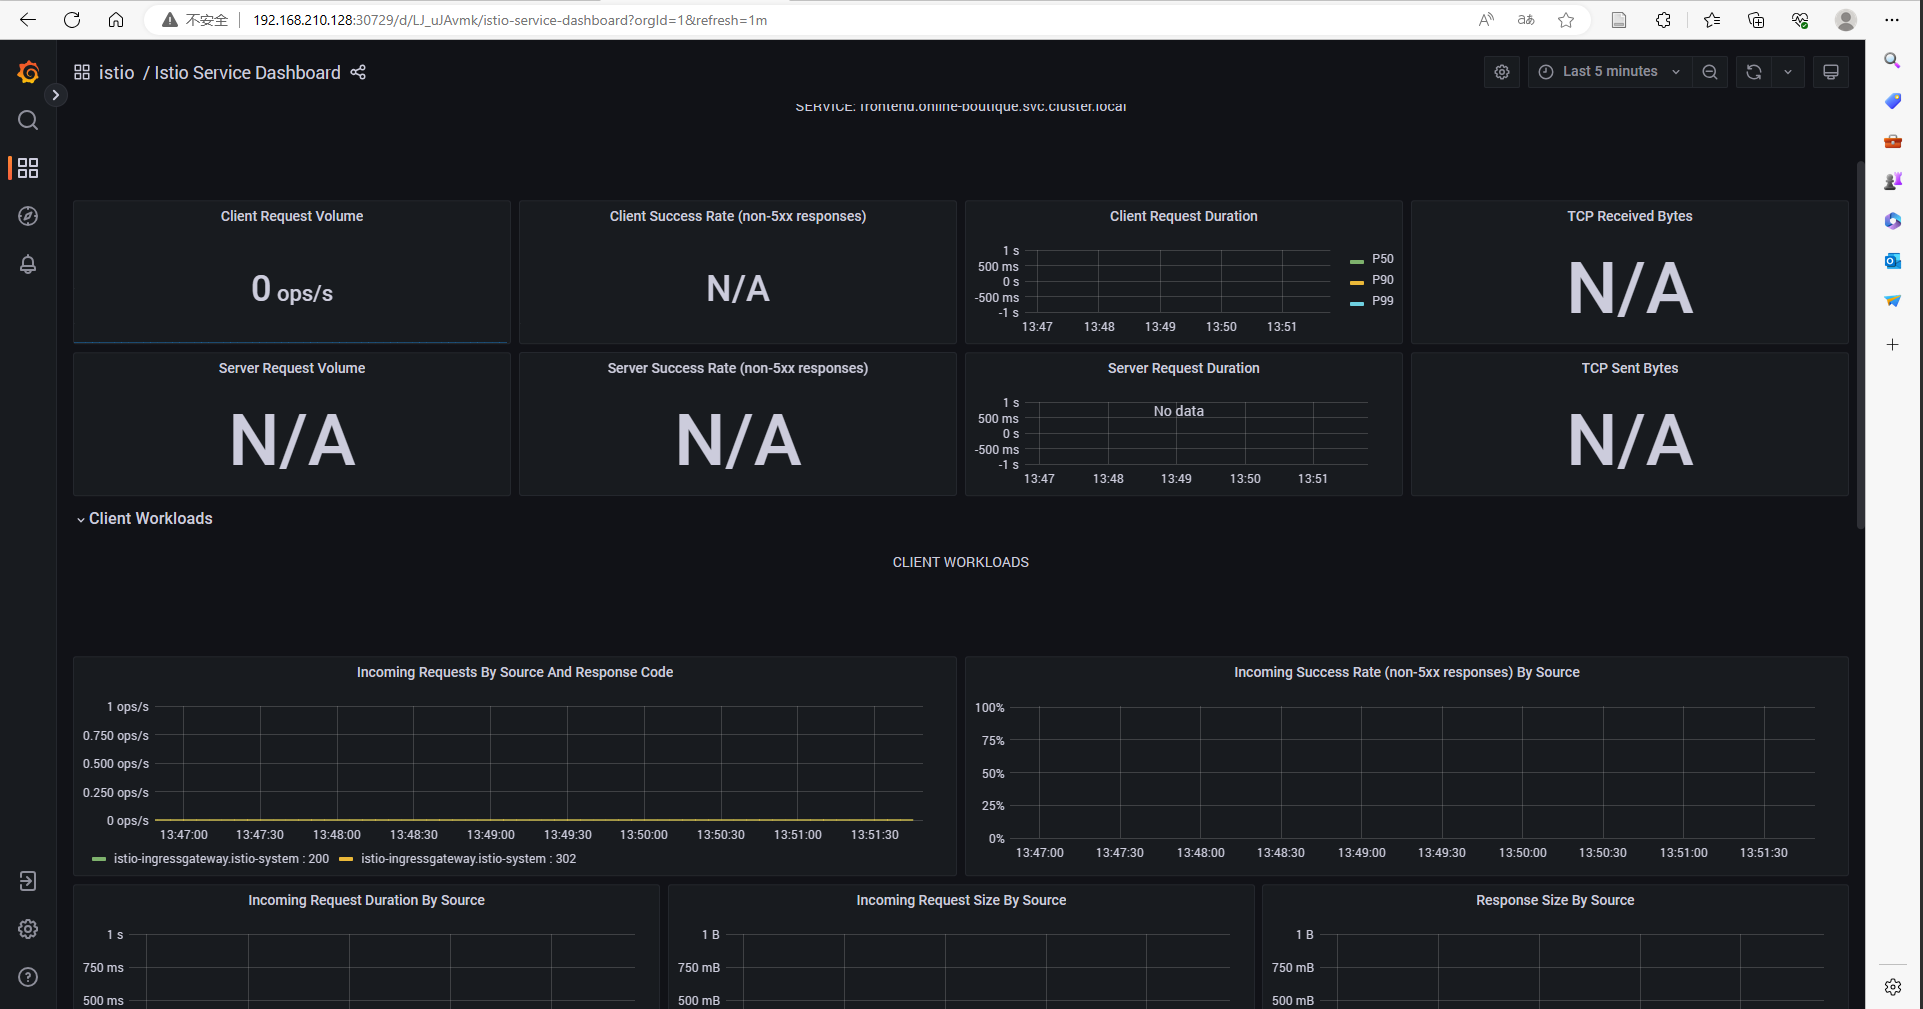
\includegraphics[width=1.0\textwidth]{figures/chapter2/SD.png}
	\caption{Istio 服务仪表盘(Istio Service Dashboard)}
	\label{fig:3-Istio 服务仪表盘(Istio Service Dashboard)}
\end{figure}
Istio Wasm 扩展仪表盘(Istio Wasm Extension Dashboard)显示与 WebAssembly 模块有关的指标,可以监控活动的和创建的 Wasm 虚拟机,关于获取删除 Wasm 模块和代理资源使用的数据。
\begin{figure}[H]
	\centering
	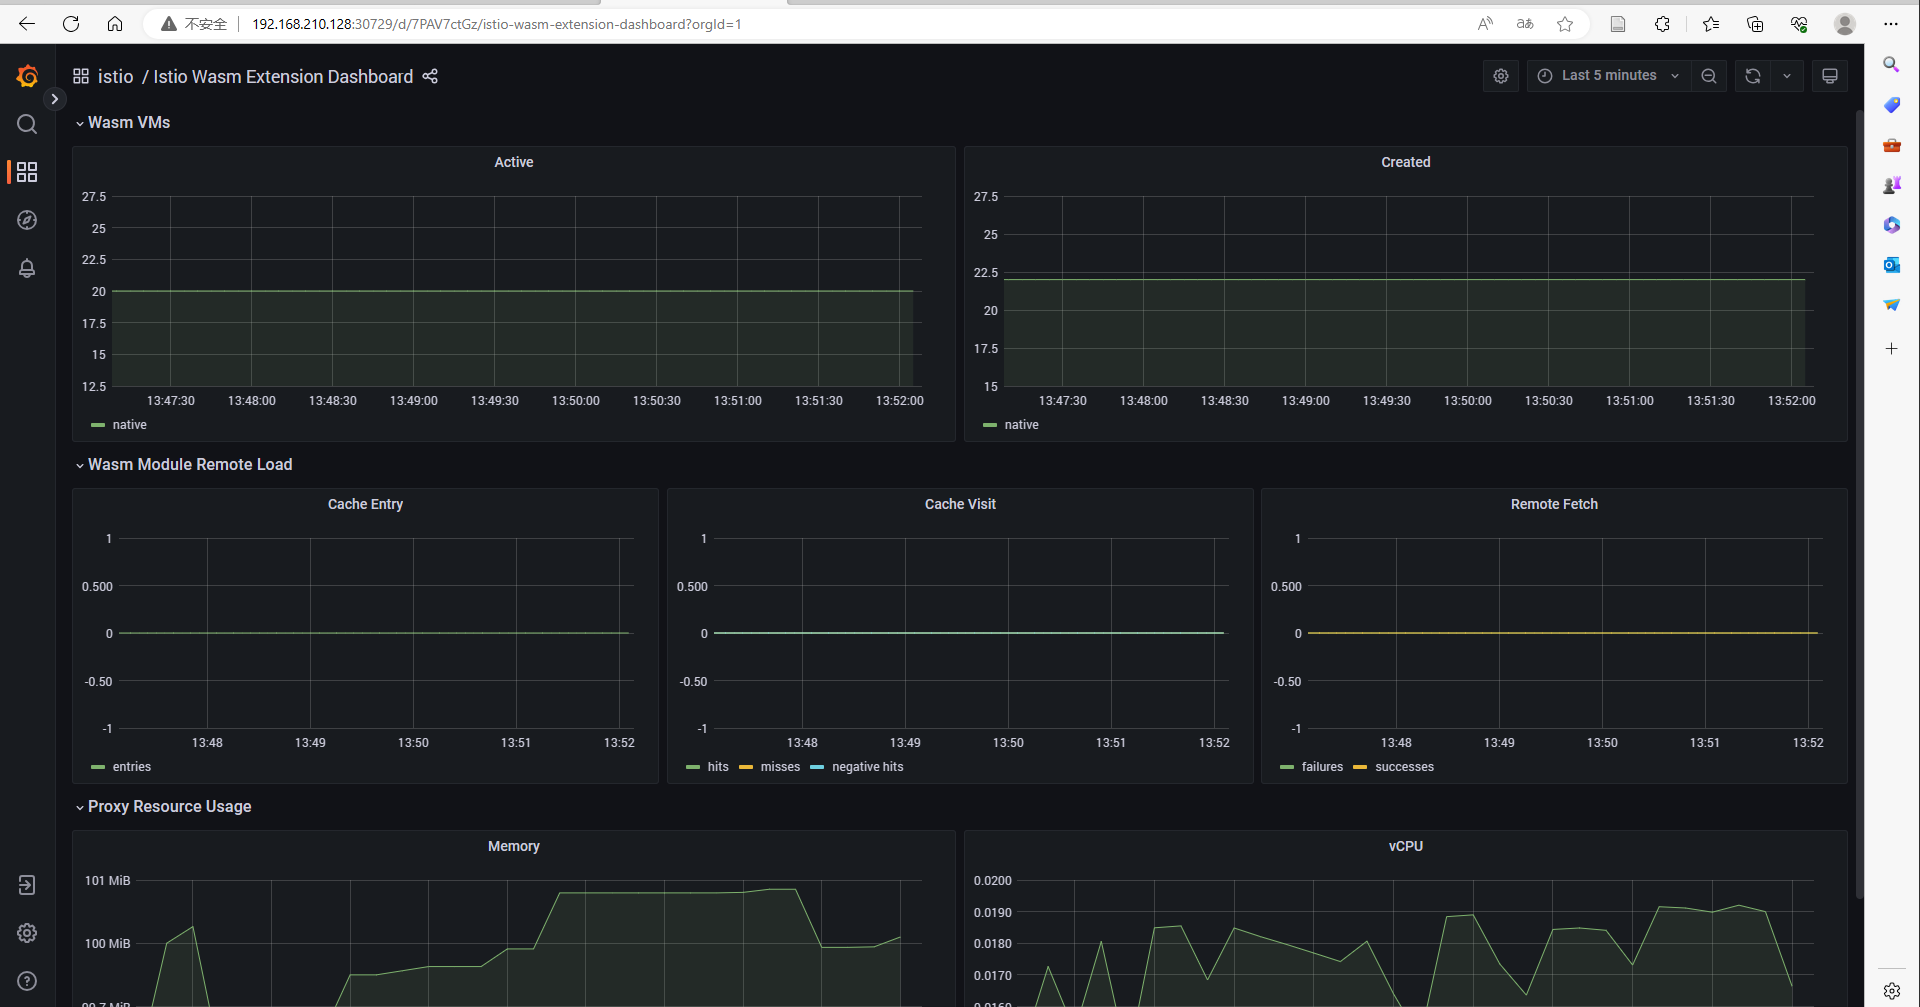
\includegraphics[width=1.0\textwidth]{figures/chapter2/WED.png}
	\caption{Istio Wasm 扩展仪表盘(Istio Wasm Extension Dashboard)}
	\label{fig:3-Istio Wasm 扩展仪表盘(Istio Wasm Extension Dashboard)}
\end{figure}
Istio 工作负载仪表盘(Istio Workload Dashboard)提供了一个工作负载的详细指标分类。
\begin{figure}[H]
	\centering
	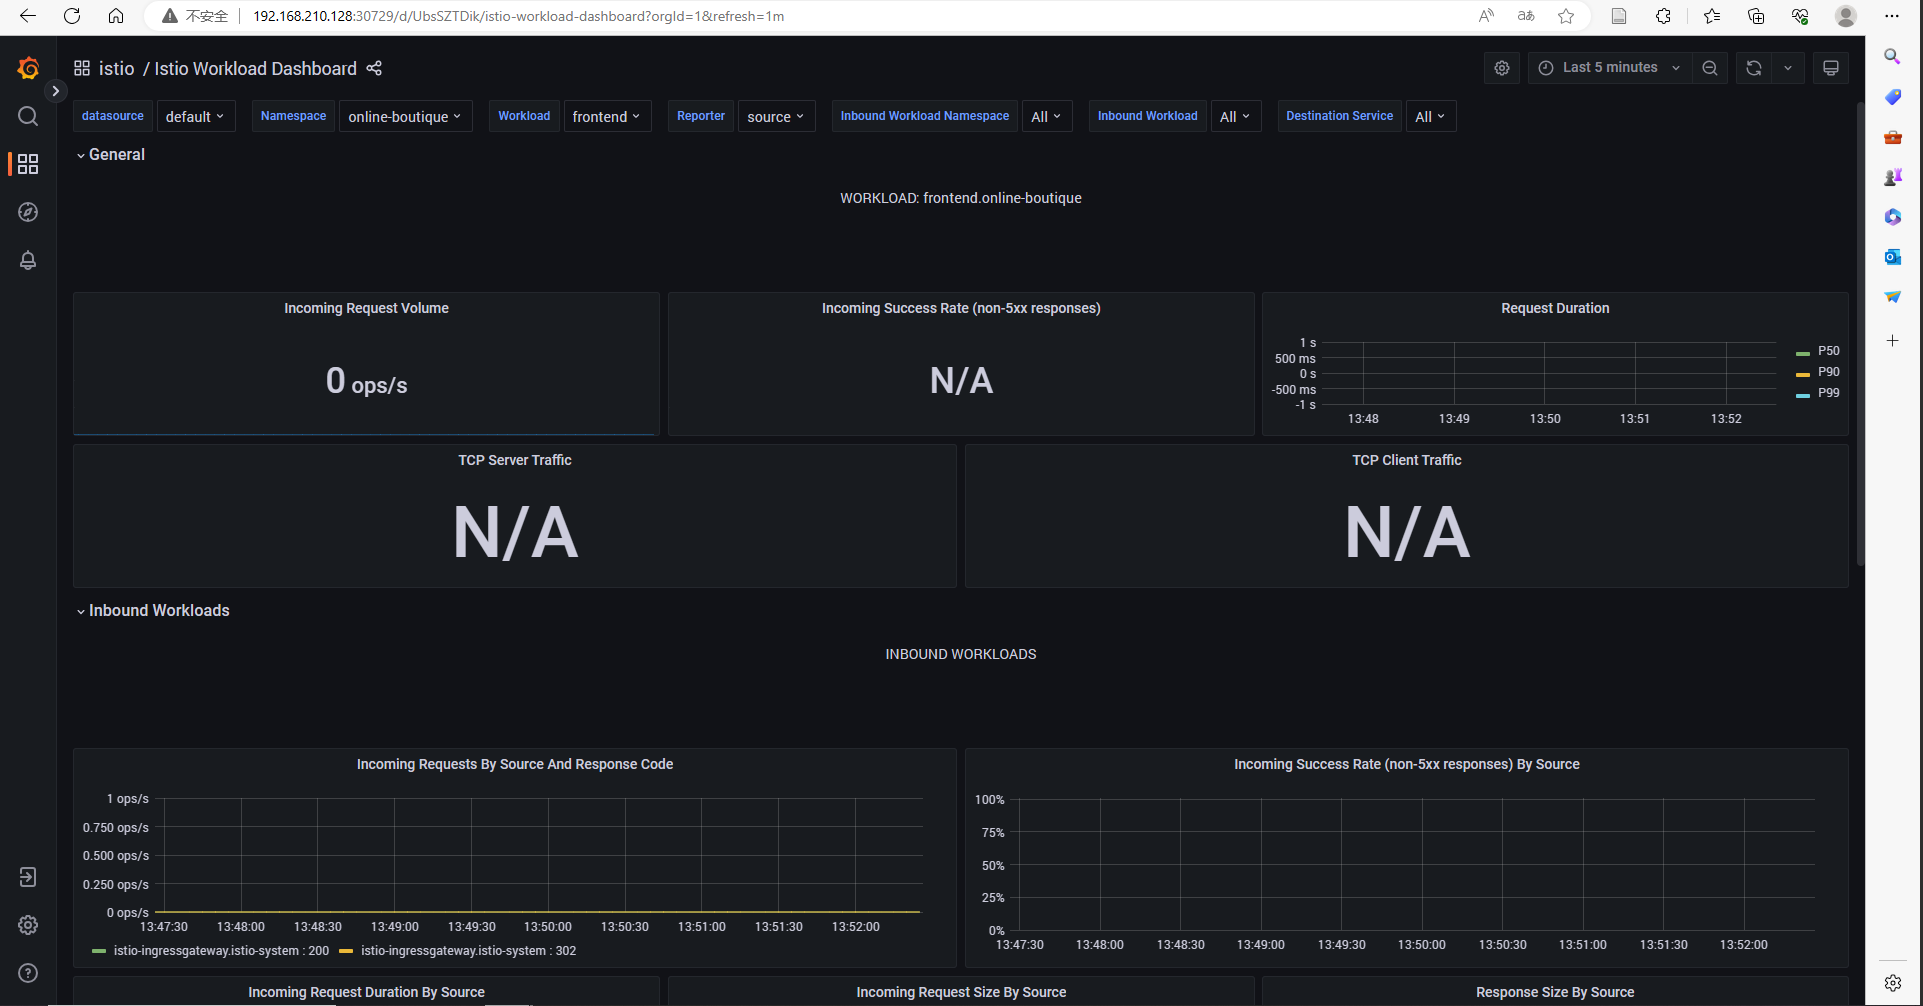
\includegraphics[width=1.0\textwidth]{figures/chapter2/WD.png}
	\caption{Istio 工作负载仪表盘(Istio Workload Dashboard)}
	\label{fig:3-Istio 工作负载仪表盘(Istio Workload Dashboard)}
\end{figure}
\section{服务拓扑发现与链路追踪}
服务拓扑发现和链路追踪是在分布式系统中实现可观测性和故障排查的关键技术。通过服务拓扑发现,我们可以了解系统中不同服务之间的依赖关系和通信流量。而链路追踪则帮助我们跟踪和分析请求在系统中的传播和处理路径,以便快速定位和解决潜在的性能问题和故障。

服务拓扑发现的目标是构建一个全面而准确的系统拓扑图,显示系统中各个服务之间的关系和依赖。它可以帮助我们了解服务之间的通信模式、调用关系以及数据流向,从而更好地理解系统的整体架构和运行方式。

链路追踪则追踪和记录请求在系统中的传播和处理路径。它通过给每个请求添加唯一标识符,并在请求经过不同的服务时进行传递和记录,以生成请求的完整链路信息。通过链路追踪,我们可以可视化请求的流程和路径,并分析每个服务的处理时间、调用关系和潜在的性能瓶颈,以便进行性能优化和故障排查。

在实际应用中,我们可以借助一些工具和平台来实现服务拓扑发现和链路追踪。其中,Kiali 和 Jaeger 是两个常用的工具,它们提供了丰富的功能和可视化界面,帮助我们监控和分析系统的服务拓扑和请求链路。

\subsection{Kiali 的配置与使用}
Kiali是一个基于Istio的服务网格管理控制台。它提供了仪表盘、可观察性,并通过强大的配置和验证能力来操作网格。Kiali可以推断流量拓扑并显示服务网格及其健康状况。Kiali提供了详细的指标、强大的验证、Grafana访问以及与Jaeger的分布式追踪的强大集成。

使用kiali.yaml文件安装kiali:
\begin{lstlisting}[language=bash]
	[root@k8scloude1 addons]# kubectl apply -f kiali.yaml
\end{lstlisting}

安装完成后,可以使用以下命令检查Kiali的部署情况:
\begin{lstlisting}[language=bash]
[root@k8scloude1 addons]# kubectl get pod -n istio-system
\end{lstlisting}

默认情况下,Kiali的Service类型为ClusterIP,无法从外部环境访问。为了让外部环境能够访问Kiali,需要将Kiali的Service类型修改为NodePort。使用以下命令编辑Kiali的Service:
\begin{lstlisting}[language=bash]
[root@k8scloude1 addons]# kubectl edit service kiali -n istio-system
\end{lstlisting}

在打开的编辑器中,将Service的类型由ClusterIP修改为NodePort,并保存更改。之后可以使用以下命令获取Kiali的Service信息:
\begin{lstlisting}[language=bash]
[root@k8scloude1 addons]# kubectl get service -n istio-system
\end{lstlisting}

在输出中,可以看到Kiali的NodePort端口号(31024)。现在,可以在浏览器中访问Kiali的网页界面。物理机IP地址为192.168.210.128,则可以在浏览器中输入以下地址:
\begin{lstlisting}[language=bash]
http://192.168.210.128:31024
\end{lstlisting}
\begin{figure}[H]
	\centering
	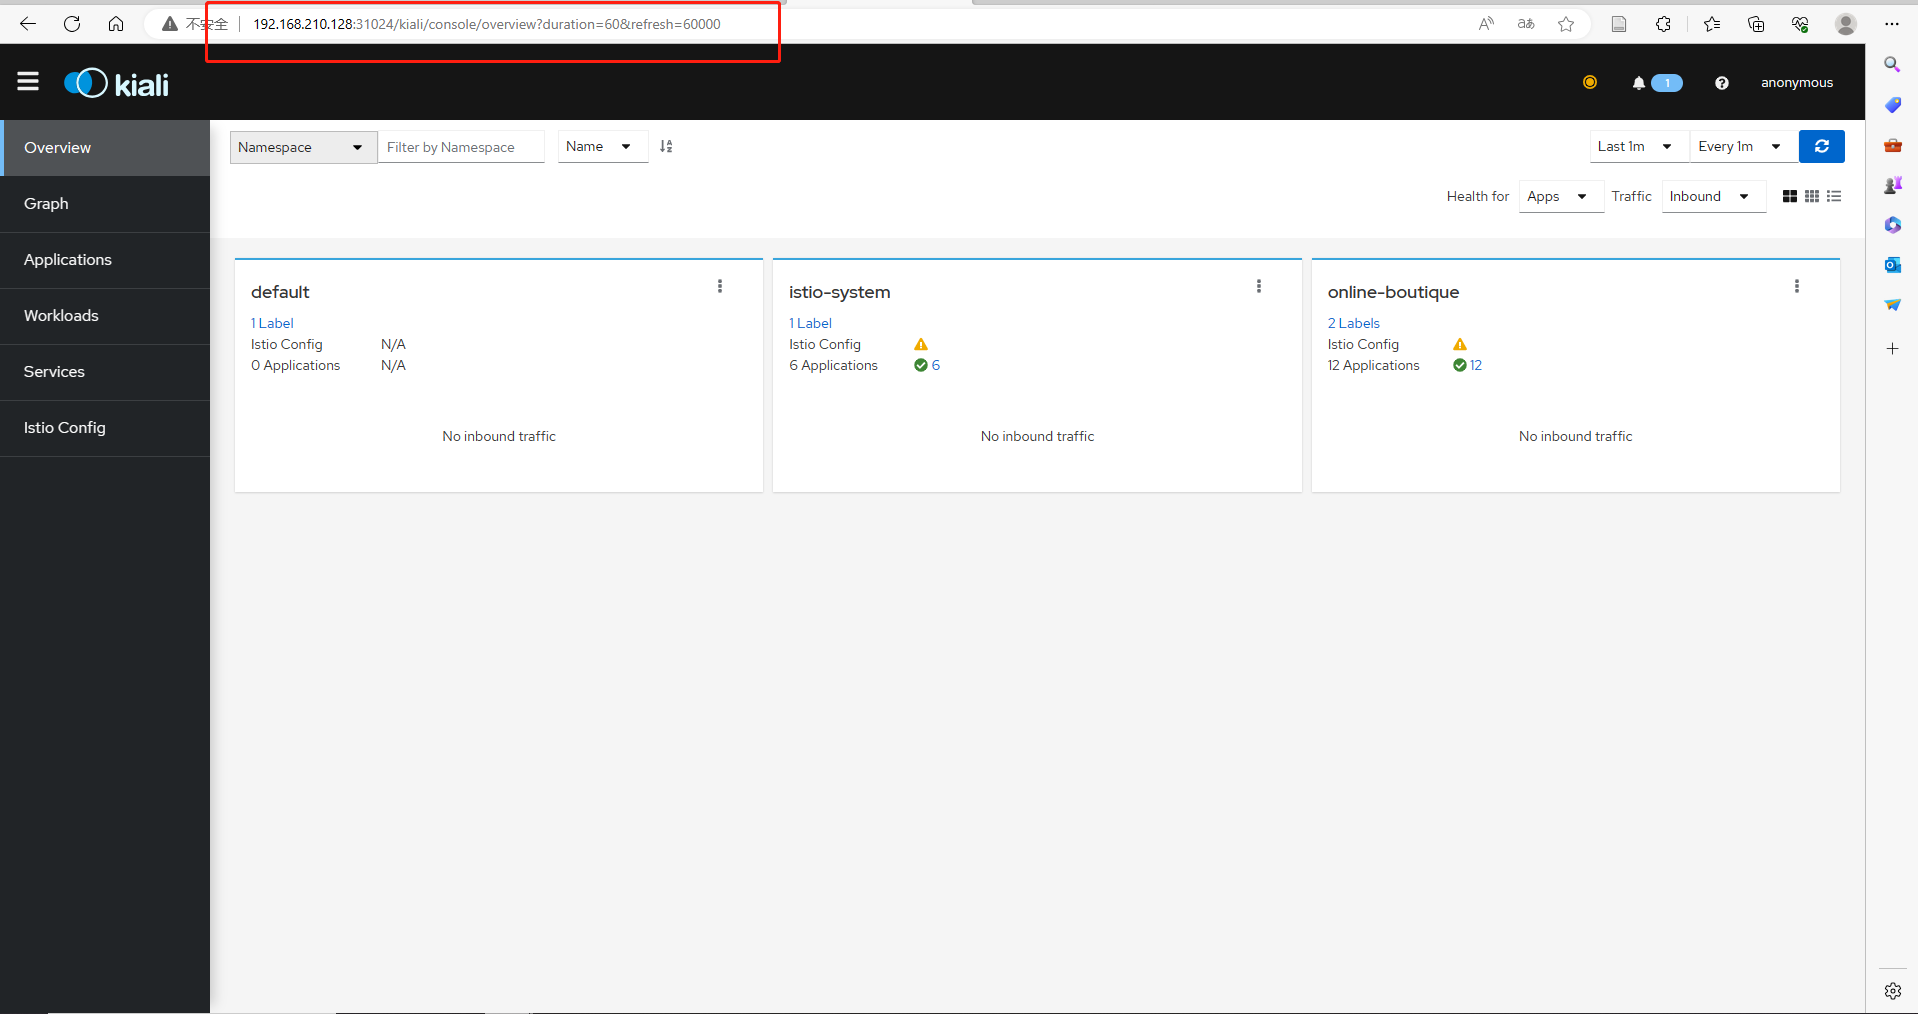
\includegraphics[width=1.0\textwidth]{figures/chapter3/kiali}
	\caption{Kiali首页}
	\label{fig:3-Kiali首页}
\end{figure}
Kiali提供了丰富的功能,使得服务网格的管理和可观察性更加便捷。
\begin{figure}[H]
	\centering
	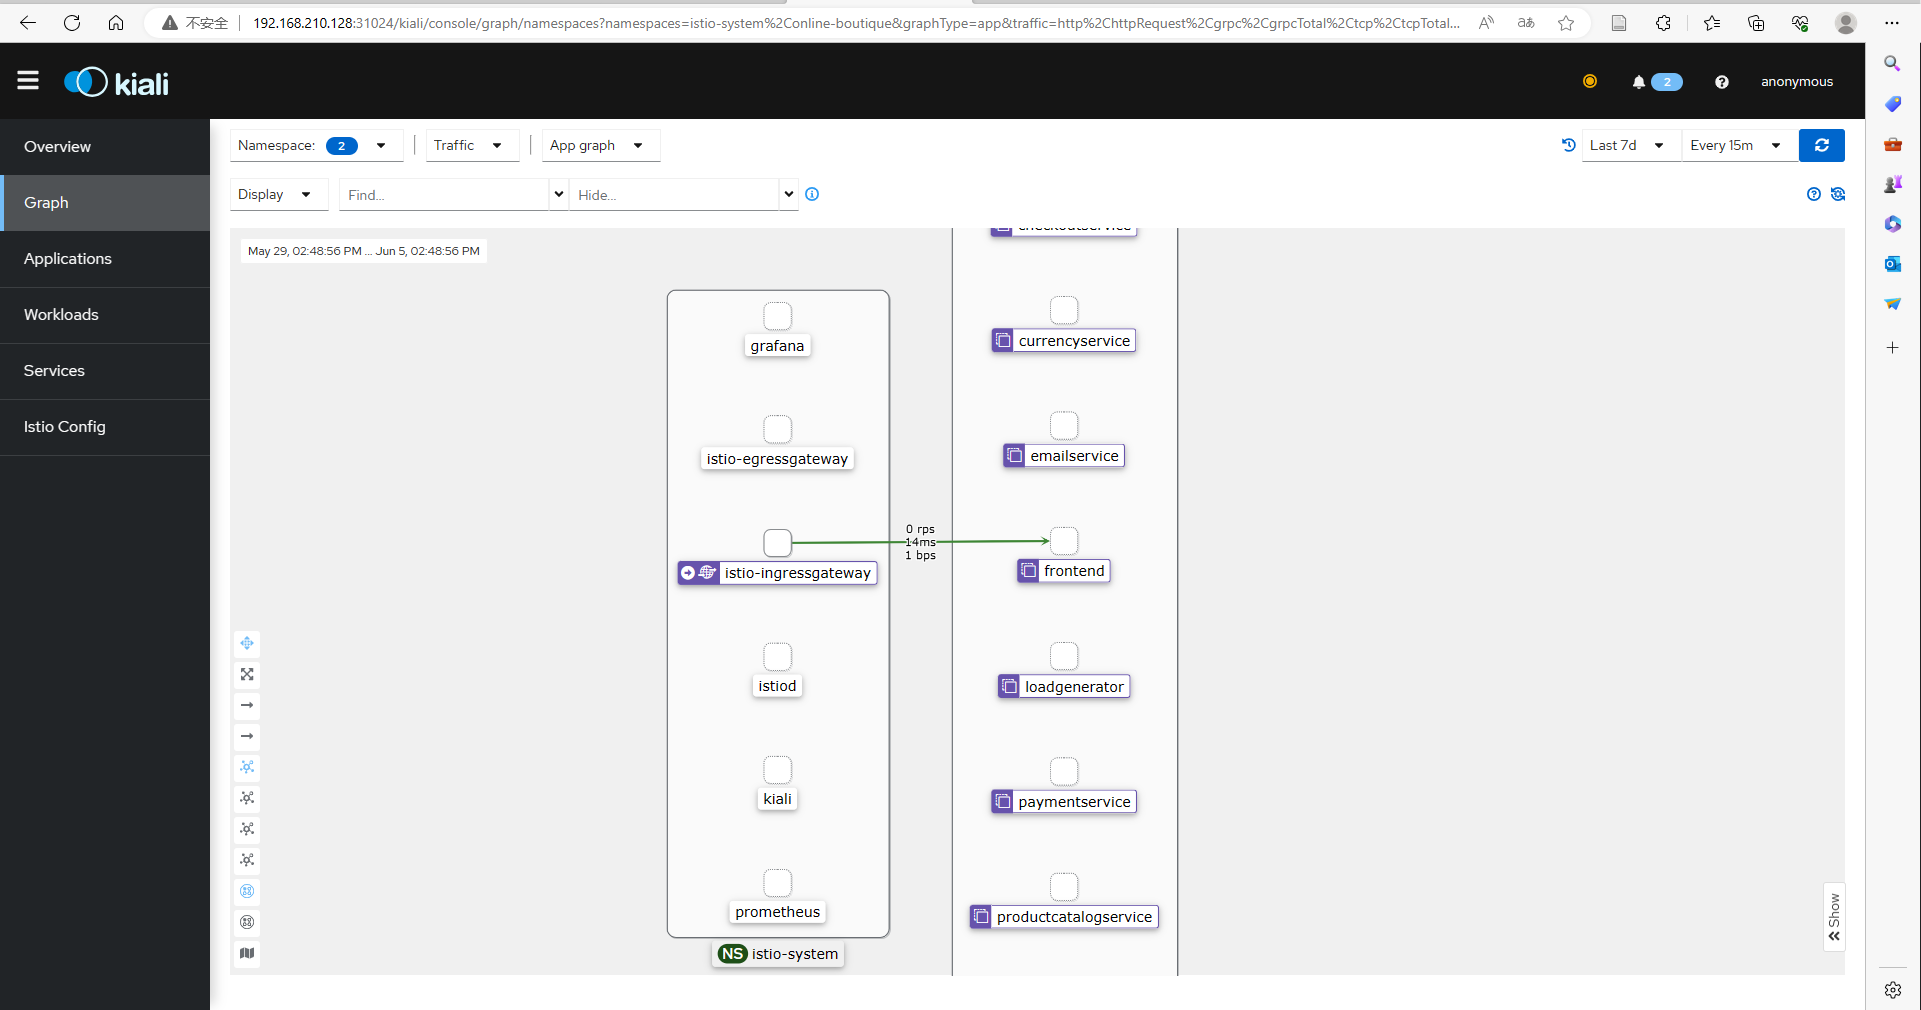
\includegraphics[width=1.0\textwidth]{figures/chapter3/online-boutique-kiali.png}
	\caption{Kiali服务拓扑图,以online-boutique为例}
	\label{fig:Kiali服务拓扑图,以online-boutique为例}
\end{figure}
Kiali生成一个服务拓扑图,展示了服务的拓扑结构,并将服务的通信方式可视化。图中的节点和边的颜色代表了服务网格的健康状况。红色或橙色的节点可能需要关注。节点的形状表示了组件的类型,如服务、工作负载或应用程序。该拓扑图还显示了入站和出站的指标,并提供与Jaeger和Grafana的集成,以便进行分布式追踪和性能监控。该图向我们展示了服务的拓扑结构,并将服务的通信方式可视化。它还显示了入站和出站的指标,以及通过连接 Jaeger 和 Grafana(如果安装了)的追踪。图中的颜色代表服务网格的健康状况。红色或橙色的节点可能需要注意。组件之间的边的颜色代表这些组件之间的请求的健康状况。节点形状表示组件的类型,如服务、工作负载或应用程序。
\begin{figure}[H]
	\centering
	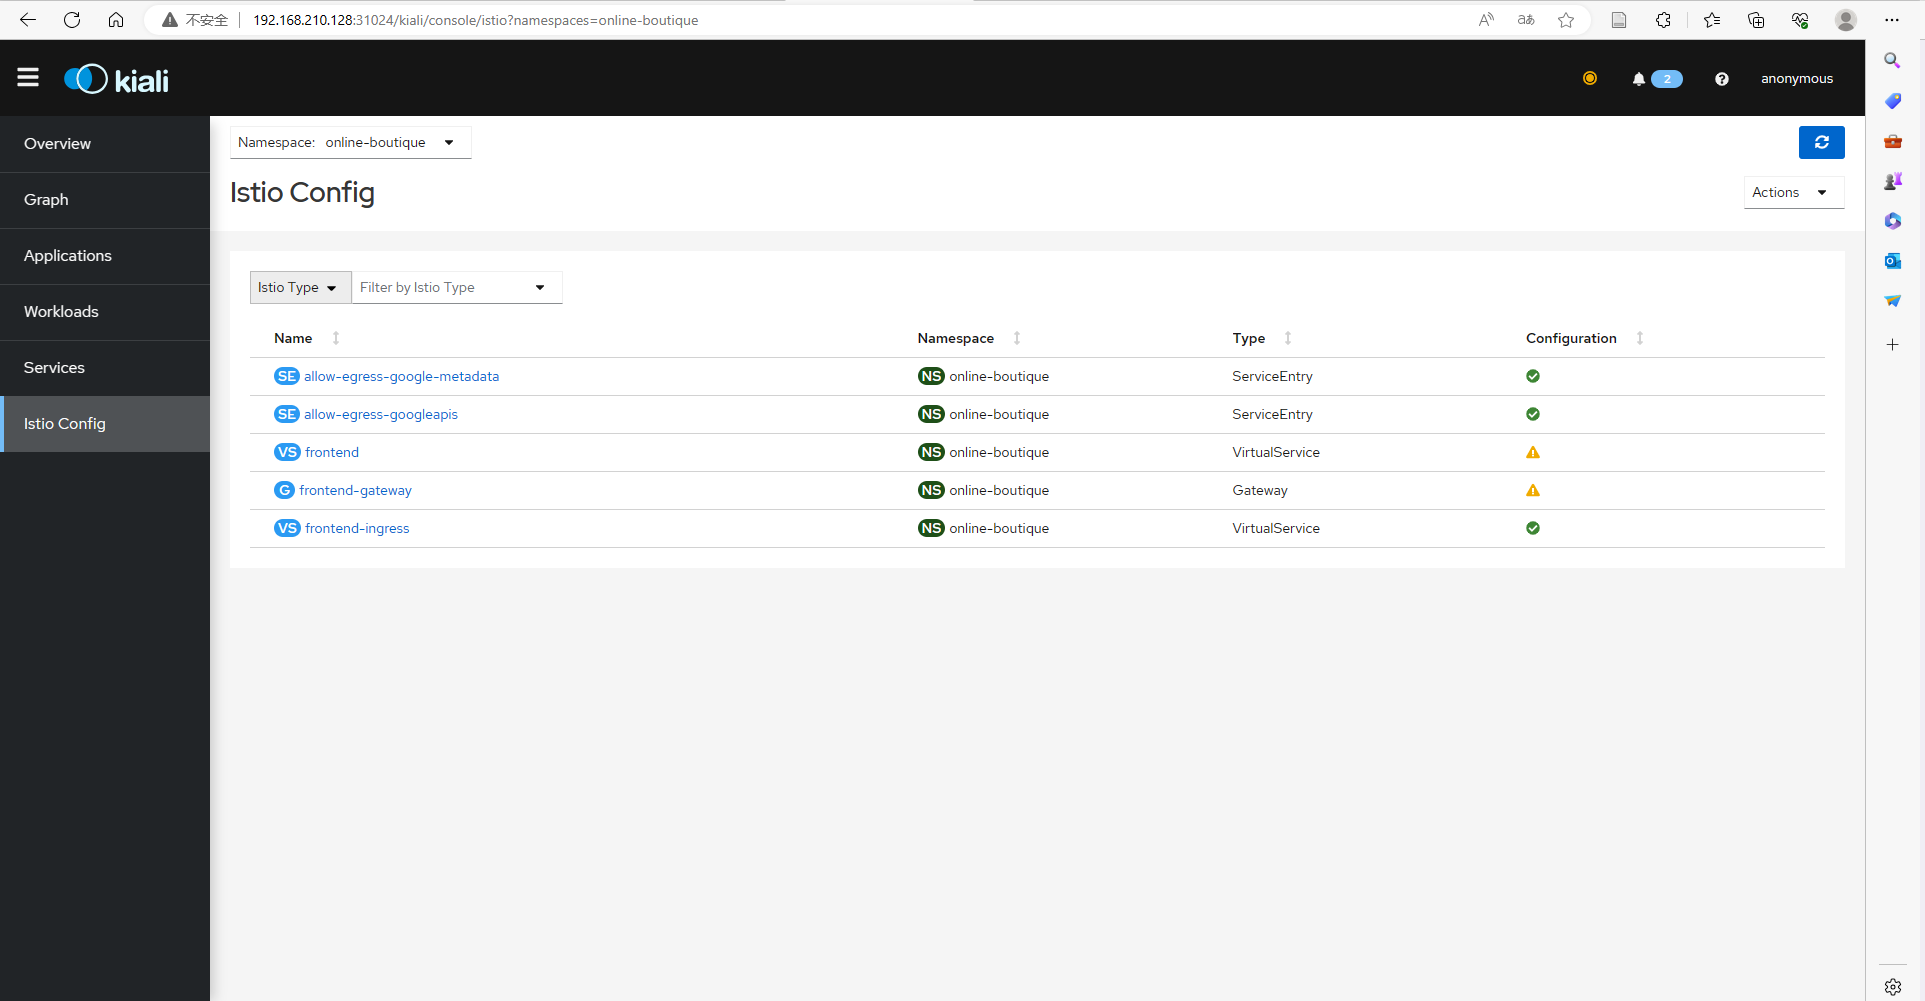
\includegraphics[width=1.0\textwidth]{figures/chapter3/kiali-config.png}
	\caption{Kiali创建、更新和删除Istio配置}
	\label{fig:3-Kiali创建、更新和删除Istio配置}
\end{figure}
Kiali允许通过向导驱动的方式创建、更新和删除Istio配置。用户可以通过Kiali界面配置请求路由、故障注入、流量转移和请求超时等功能。如果已经部署了现有的Istio配置,Kiali可以验证配置并报告任何警告或错误。Kiali的配置操作使得管理和调整服务网格变得更加直观和方便。通过Kiali,可以更好地管理和可视化服务网格,并进行配置和验证操作。同时,Kiali还提供了与Jaeger和Grafana等工具的集成,为分布式追踪和性能监控提供了便利。

\subsection{Jaeger 的配置与使用}
Jaeger是一个开源的分布式追踪系统,用于监控和故障排查分布式应用程序。它提供了端到端的追踪,使开发人员能够可视化请求在系统中的传播和处理路径,并识别潜在的性能瓶颈和故障点。

在分布式系统中,由于请求涉及多个服务和组件之间的相互作用,跟踪请求的流程和了解其在系统中的行为变得非常重要。Jaeger通过在分布式应用程序中插入轻量级追踪代码,收集跨服务边界的时间数据,以及请求在各个组件之间的传播路径和执行时间,从而提供了对应用程序性能和行为的深入洞察。

Jaeger提供了一个用户友好的界面,展示了请求的跟踪数据,包括请求的开始和结束时间、各个组件的处理时间、请求在组件之间的流转情况等。这些信息对于识别性能瓶颈、故障排查和系统优化非常有价值。

通过集成Jaeger客户端库和相关的追踪API,开发人员可以在他们的应用程序中生成和发送追踪数据给Jaeger进行分析。Jaeger提供了丰富的工具和API,以支持各种编程语言和框架,使开发人员能够轻松地将追踪功能集成到他们的应用程序中。

总而言之,Jaeger是一个强大的分布式追踪系统,为开发人员提供了对分布式应用程序的可观测性,帮助他们理解和优化应用程序的性能和行为。


使用jaeger.yaml文件安装Jaeger:
\begin{lstlisting}[language=bash]
	[root@k8scloude1 addons]# kubectl apply -f jaeger.yaml
\end{lstlisting}

安装完成后,可以使用以下命令检查Jaeger的部署情况:
\begin{lstlisting}[language=bash]
	[root@k8scloude1 addons]# kubectl get pod -n istio-system
\end{lstlisting}

默认情况下,Jaeger的Service类型为ClusterIP,无法从外部环境访问。为了让外部环境能够访问jaeger,需要将Jaeger的Service类型修改为NodePort。使用以下命令编辑Jaeger的Service:
\begin{lstlisting}[language=bash]
	[root@k8scloude1 addons]# kubectl edit service jaeger-collector -n istio-system
\end{lstlisting}

在打开的编辑器中,将Service的类型由ClusterIP修改为NodePort,并保存更改。之后可以使用以下命令获取Jaeger的Service信息:
\begin{lstlisting}[language=bash]
	[root@k8scloude1 addons]# kubectl get service -n istio-system
\end{lstlisting}

在输出中,可以看到Jaeger的NodePort端口号30038,可以在浏览器中访问Jaeger的网页界面。物理机IP地址为192.168.210.128,则可以在浏览器中输入以下地址:
\begin{lstlisting}[language=bash]
	http://192.168.210.128:30038
\end{lstlisting}